\chapter{Research projects}%
	\label{ch:paper}

\newthought{The research project} is the graded coursework component that you will work on with a student partner throughout the entire semester. It consists in regularly submitting a draft paper with its replication script, in the form of a Stata do-file.

In the first half of the course, you will submit and revise the \emph{first draft} of your project. The exact deadline for submission will be discussed in class. More important is the overall planning that you will have to follow until then:

\begin{enumerate}
  \item In Week~1, explore the course datasets.
  \item In Week~2, register yourself in the class projects list.
  \item In Week~3, register your \emph{group} in the class projects list.
  \item In Week~4, download the first draft template.
  \item In Week~5, submit your first draft.
  \item In Week~6, correct your first draft.
\end{enumerate}

In the second part of the course, you will resubmit a \emph{revised draft}, and then finally hand in your \emph{final paper} by the end of the course. The final deadline is generally set to ``Week~13'', one week after the last course session.

\section{Principles}

Keep it simple. Choose a simple opening line that states the most salient characteristic of the issue under scrutiny. ``Cancer commissioning is complex'' or ``Survey weighting is a mess'' are both real, and acceptable, examples.

\subsection{Parsimony}

Substantively, your model is about explaining some relationships between social forces. Statistically, it is about understanding variance by predicting it. for your paper, select only what is needed from your statistical analysis to test your substantive theory. Leave the `tech specs' in your do-file, with comments in the source, and aim at writing an argument that will be based on your expertise rather than on computer code.%

  Be parsimonious in your approach to modeling: select your findings to the bare logical minimum required by your analysis. Your do-file will contain tons of tests and models, but do not publish every intermediate result that was taken in your analysis: report statistically significant findings for which you can provide an interpretation, and document negative results when they are surprising with reference to your hypotheses.%

\paragraph{Tables and numbers} Even in a quantitative environment, you should feel some pressure to reduce the number of numbers in your work to their bare minimum. There are only a few requirements, such as summary statistics or regression estimates. In many circumstances, you might want to leave any other result in your do-file. This, for instance, applies to several crosstabulations that you might have run until now, although you can cite particular percentages or tests.%

  A simple example of parsimony in numbers concerns precision. Many social science measurements have no serious degree of precision: measures of social attitudes, for example, are taken on 11-point scales at most. If you report value with a lot of digits after the decimal separator, as in \texttt{8.4759}, you are suggesting that your data are reliable at that level of precision, which is very rarely true. Round up, therefore, all numbers to 0, 1 or 2 decimals.%

\paragraph{Figures} It is an excellent idea to visually inspect the distributions and relationships in your data, as it is to use graphs where tables could have done but would have conveyed less information to the reader.%

  Make sure, however, to include figures only when they bring more information than you can efficiently convey in a few sentences. Your do-file contains a lot of graphic output, and you will have to select figures based on that assessment.%

  Make, therefore, a \emph{very} restricted choice of plots. Include them at the end of the manuscript, and refer to them by their figure number.%

  You might want to use some Stata graph options to enhance your plots before exporting them for inclusion in your paper. Make sure, for instance, to set axis labels with the \coab{xti}{xtitle}{graph} and \coab{yti}{ytitle}{graph} options and comprehensible value labels.%

\paragraph{Significance tests} Remember that the principle of statistical significance is to estimate the probability level of the null hypothesis, i.e. an abstract situation where, to make it simple, the variations in your data are compared to the absence of any significant variation. `Rejecting the null' is actually often trivial: you will always find some covariance in social data, even if it is completely spurious and/or statistically powerless.%

  For these reasons, report $p$-values in your text only when you feel that the reader might want to see it: if you are making an important claim, or if you are interpreting a coefficient or test with a high $p$-value but which you still believe to be significant (recall what was mentioned several times about the freedom of judgement that you should exert around the conventional boundary of $p < .05$).%

\subsection{Validity}

\begin{quote}
	We all know that art is not truth. Art is a lie that makes us realize truth, at least the truth that is given us to understand. The artist must know the manner whereby to convince others of the truthfulness of his lies. (The Arts, \emph{Picasso Speaks}, 1923)\footnote{Cited in \href{http://languagelog.ldc.upenn.edu/nll/?p=3103}{Mark Liberman, ``Gelman and Picasso'', \emph{Language Log}, 9 June 2011}.}
\end{quote}

Your research question and your statistical model are tied together. 

\paragraph{Measurement validity} When ``measurable data are not accurate representations of their underlying constructs'' (p.~293), models can only provide a conceptual view of what is occurring in the real world.\footnote{\href{http://projecteuclid.org/euclid.ss/1294167961}{\fullcite{Shmueli:2010a}}.}

\paragraph 

\paragraph{Kitchen-sink models}. Achen.  \href{http://polmeth.wustl.edu/mediaDetail.php?docId=1246}{\fullcite{Schrodt:2011a}}. `Type III error' is when your model brings the right answer to the wrong question.%
     %
     \footnote{Originally from Peter Kennedy's ``The Ten Commandments of Applied Econometrics,'' cited by Christopher S.~McIntosh at \url{http://courses.cals.uidaho.edu/aers/agecon525/sp2010/Lecture21DoingAppliedEconometrics.pdf}.} %
     %
     Don't control, stratify.

\paragraph{Weak effects} Weak effects are statistically significant coefficients that are very weakly transformative of the dependent variable and therefore end up being disappointing at the substantive level, as in: `an infinitesimal variation in $x$ that would be barely noticeable in real settings causes a statistically robust but empirically negligible variation in $y$'.%

  % The magnitude of the effects in your model should be your only benchmark to determine how substantively significant your findings are. Statistical significance is, in many ways, less of a concern: a statistically insignificant result might just need a larger sample to be observed, while a trivial effect size might not adjust to expectations, regardless of the sample size.%

  % This perspective implies that in your hands, the main interest of a statistical model lies in effect size rather than in predictive capacity or statistical significance. Confidence intervals should carry enough information for you to judge how precisely you have measured an effect, and the interpretation of the size of the effect is where ...%

  % In the case where a predictor is `under-performing' in your model, it might simply be that linear regression is not the most appropriate method for your data, which is a perfectly acceptable conclusion if you can explain why it was not possible to capture the relationship under scrutiny with a linear regression model.%
  
  % In the case where your dependent variable is susceptible to be central to the issue, you are advised to consider recoding it to a binary variable and switch to logistic regression.%

\paragraph{Negative results} Your model might return negative results, i.e. findings that directly contradict your hypotheses. This happens when a variable predicted as having a strong positive effect is estimated to have a strong negative effect, or vice versa.%

  If you detect negative results in your findings, start by rechecking your model specifications. If your hypothesis seems seriously at risk, reconsider the functional form of your model (should it be linear?), as well as the functional form of your hypothesis (e.g. increasing returns and returns to scale).%

%

\section{Formatting}

\newthought{This section} shows how to produce the tables mentioned in the paper template. The examples below use variables from the \qog{} dataset:%

\begin{verbatim}
// example data
use bl_lu_25mf undp_gii wvs_abort wvs_theo unna_pop wdi_gdpc using data/qog2013, clear
// log-transformations
gen log_pop = ln(unna_pop)
la var log_pop "Log(Population)"
gen log_gdpc = ln(wdi_gdpc)
la var log_gdpc "Log(GDP per capita)"
\end{verbatim}

%
\paragraph{Summary statistics}%
  \index{Descriptive statistics!Table formatting}%
  %
  The \cmd{stab} program, which is part of the course setup that you ran at p.~\pageref{sec:course-setup}, lets you export plain text tab-separated tables of summary statistics. These tables are convenient to open in spreadsheet editors like Microsoft Excel or OpenOffice Calc, and can be pasted into Google Documents.%

  %
  The \cmd{stab} command is a wrapper for some of the export functions in the \cmd{estout} package. There are clunkier ways to export summary statistics in more sophisticated ways with \cmd{tabout} and its supplementary command \opt{tabstatout}{tabout}, but you should be fine with \cmd{stab}.%

%
\paragraph{Correlation matrix}%
  \index{Correlation!Matrixes}%
  %
  Table~\ref{tbl:estout-corr} shows a correlation matrix exported with the \cmd{estout} package, as shown at p.~\pageref{tbl:correlate_export}.%

  %
  % The numbering system saves space on paper, and columns are aligned on the decimal point to increase readability. Variable labels are preferable to less informative variable names. Last, remember to stick a complete caption. \emph{Note:} if you want to use cell colors to `warm up' the table, please feel free to do so, using a soft color theme.
  %
\begin{fullwidth}
	\begin{table}
		\footnotesize
    %
    {
\def\sym#1{\ifmmode^{#1}\else\(^{#1}\)\fi}
\begin{tabular}{l*{8}{c}}
\hline\hline
                &\multicolumn{8}{c}{}                                                                                                                                   \\
                &(1)&(2)&(3)&(4)&(5)&(6)&(7)&(8) \\
\hline
(1) No Schooling, Female and Male (25+)&        1         &                  &                  &                  &                  &                  &                  &                  \\
(2) Gender Inequality Index&    0.744\sym{***}&        1         &                  &                  &                  &                  &                  &                  \\
(3) Population      &    0.221         &    0.269         &        1         &                  &                  &                  &                  &                  \\
(4) GDP per Capita, PPP (Constant International USD)&   -0.606\sym{***}&   -0.828\sym{***}&   -0.121         &        1         &                  &                  &                  &                  \\
(5) Abortion is justifiable&   -0.517\sym{***}&   -0.729\sym{***}&  -0.0934         &    0.750\sym{***}&        1         &                  &                  &                  \\
(6) Support for theocracy&    0.579\sym{***}&    0.834\sym{***}&   0.0952         &   -0.763\sym{***}&   -0.865\sym{***}&        1         &                  &                  \\
(7) Log(Population) &    0.125         &    0.255         &    0.621\sym{***}&   -0.140         &   -0.274         &    0.219         &        1         &                  \\
(8) Log(GDP per capita)&   -0.762\sym{***}&   -0.835\sym{***}&   -0.143         &    0.903\sym{***}&    0.648\sym{***}&   -0.700\sym{***}&   -0.106         &        1         \\
\hline
Observations    &       41         &                  &                  &                  &                  &                  &                  &                  \\
\hline\hline
\multicolumn{9}{l}{\footnotesize \sym{*} \(p<0.05\), \sym{**} \(p<0.01\), \sym{***} \(p<0.001\)}\\
\end{tabular}
}

		%
		\caption{Correlation output produced with \cmd{estout} and edited by adding variable numbers.}
		\label{tbl:estout-corr}
	\end{table}
\end{fullwidth}

\begin{verbatim}
// export correlation matrix with -estout-
keep wvs_abort bl_lu_25mf log_*
qui estpost correlate *, matrix listwise
esttab using correlates.csv, replace unstack not compress label nonum
\end{verbatim}

%
%
%
\index{Linear regression!Exporting results}
\paragraph{Regression estimates}

Table~\ref{tbl:hibbs_yx1_predict} shows how to pass several \cmmd{predict} commands to store some estimates. We store the fitted values under the name \texttt{yhat} in reference to $\hat{Y}$, the estimated values of the dependent variable $Y$: for every $i=1, \ldots, n$ observations, $Y_i = \hat{Y_i} + \epsilon_i$. To store the residuals in the units of the dependent variable, we use \cmmd{predict} with the \coab{resid}{residuals}{predict} option. The standardized residuals, calculated in standard deviations of their own distribution, are stored with the \coab{rsta}{rstandard}{predict} option.

\begin{table}[htp]
	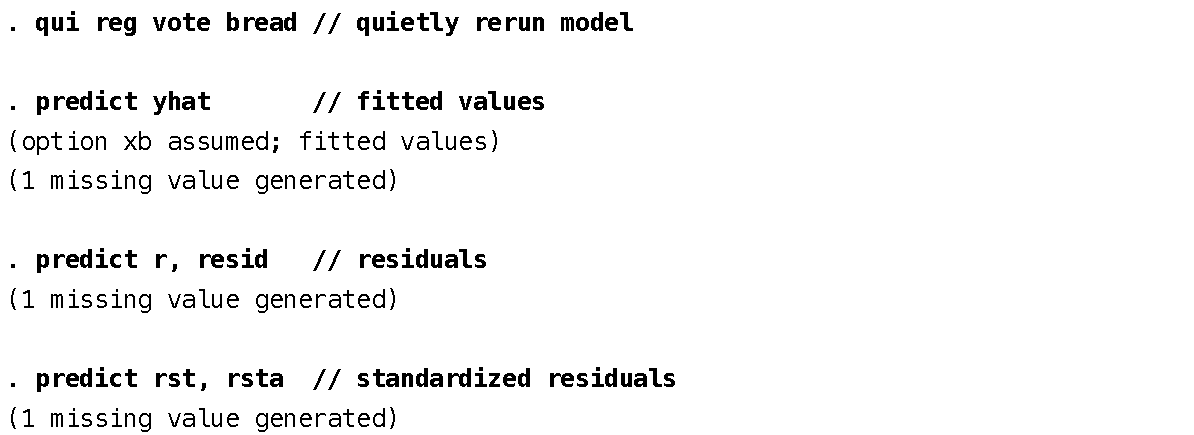
\includegraphics[scale=.5]{figures/hibbs_yx1_predict.pdf}

	\caption[Storing estimates with \cmmd{predict}]{\label{tbl:hibbs_yx1_predict}
	Storing estimates with \cmmd{predict}.\\
	\hibbs{15}}
\end{table}%

Prior to interpreting the content of the regression table/output, a good idea is to take care of saving the model results straight away, in simplified format.

Table~\ref{tbl:estout-reg} shows regression output exported with \cmd{estout} as shown at p.~\pageref{tbl:hibbs_yx1_estout}. Models are each in a separate column with a short title, and a lot of information has been dropped to reflect the most relevant aspects of the model. If you need more sophisticated output, Ben Jann's online documentation for \cmd{estout} contains useful examples.%
\footnote{\url{http://repec.org/bocode/e/estout/index.html}.}

% If you are focusing on standardized coefficients, you can produce an even more simplified output with the \opt{beta}{esttab} and \texttt{not} options.

\begin{fullwidth}
	\begin{table}
		\footnotesize
    %
    {
\def\sym#1{\ifmmode^{#1}\else\(^{#1}\)\fi}
\begin{tabular}{l*{4}{c}}
\hline\hline
                    &\multicolumn{1}{c}{(1)}&\multicolumn{1}{c}{(2)}&\multicolumn{1}{c}{(3)}&\multicolumn{1}{c}{(4)}\\
                    &\multicolumn{1}{c}{Full model}&\multicolumn{1}{c}{Controls}&\multicolumn{1}{c}{Theocracy}&\multicolumn{1}{c}{GII}\\
\hline
No Schooling, Female and Male (25+)&         0.0         &        -0.0         &         0.0         &         0.0         \\
                    &       (0.0)         &       (0.0)         &       (0.0)         &       (0.0)         \\
[1em]
Log(Population)     &        -0.1         &        -0.2         &        -0.1         &        -0.1         \\
                    &       (0.1)         &       (0.1)         &       (0.1)         &       (0.1)         \\
[1em]
Log(GDP per capita) &         0.3         &         1.0\sym{***}&         0.2         &         0.4         \\
                    &       (0.3)         &       (0.2)         &       (0.2)         &       (0.3)         \\
[1em]
c.undp\_gii#c.wvs\_theo&       -10.2\sym{**} &                     &                     &                     \\
                    &       (3.0)         &                     &                     &                     \\
[1em]
Support for theocracy&                     &                     &       -10.5\sym{***}&                     \\
                    &                     &                     &       (1.7)         &                     \\
[1em]
Gender Inequality Index&                     &                     &                     &        -4.8\sym{**} \\
                    &                     &                     &                     &       (1.6)         \\
[1em]
Constant            &         4.4         &        -1.7         &         8.6\sym{**} &         3.3         \\
                    &       (3.3)         &       (3.1)         &       (2.7)         &       (3.4)         \\
\hline
Observations        &          41         &          49         &          42         &          48         \\
rmse                &         1.0         &         1.2         &         0.8         &         1.1         \\
\hline\hline
\multicolumn{5}{l}{\footnotesize Standard errors in parentheses}\\
\multicolumn{5}{l}{\footnotesize \sym{*} \(p<0.05\), \sym{**} \(p<0.01\), \sym{***} \(p<0.001\)}\\
\end{tabular}
}

		%
		\caption{Regression output produced with \cmd{estout}.}
		\label{tbl:estout-reg}
	\end{table}
\end{fullwidth}

To produce this example, we first stored some example specifications of a linear regression model into short names \texttt{m1} to \texttt{m4}. To store a model, simply prefix its command with \texttt{eststo (name): qui}, which will quietly run the model and save it under \texttt{(name)}:

\begin{verbatim}
// example models
eststo m1: qui reg wvs_abort bl_lu_25mf log_* c.undp_gii#c.wvs_theo
eststo m2: qui reg wvs_abort bl_lu_25mf log_*
eststo m3: qui reg wvs_abort bl_lu_25mf log_* wvs_theo
eststo m4: qui reg wvs_abort bl_lu_25mf log_* undp_gii
\end{verbatim}

Note that the full model has an interaction term, and that the three other models simply show how the model behaves under slightly different specifications. The entire output is exported with a single command, \cmd{esstab}:

\begin{verbatim}
// export regression output with -estout-
esttab m1 m2 m3 m4 using models.csv, ///
  replace label b(1) se(1) sca(rmse) ///
	mti("Full model" "Controls" "Theocracy" "GII")
\end{verbatim}

The \texttt{b(1)} and \texttt{se(1)} options set the unstandardised coefficients and standard errors to one digit precision. The \texttt{sca(rmse)} option adds the RMSE to each model, for which names are set by the \texttt{mti} option.
